\part{Engine: Aufbau}

Ein Spiel innerhalb der Web-Engine besteht aus verschiedenen Komponenten. Zunächst existiert eine \textprog{entry.js}-Datei, welche den Startpunkt des Spiels bestimmt. Innerhalb dieser werden die für bestimmte Aufgaben (Grafik, Physik, Input, Audio) zuständigen \textbf{Manager} erzeugt und konfiguriert. Diese sind global aus allen Teilen des Programmcodes erreichbar. Zusätzlich wird eine \textbf{Instanz der Spielklasse} erstellt, welche ebenfalls global erreichbar ist.

\todo{Illustration}

\chapter{GameCore}

Der Kern eines Spiels befindet sich innerhalb einer vom Programmierer erweiterten (oder geerbten) Instanz der Klasse \textprog{BaseGame}. Diese Klasse beherbergt Funktionen zum Laden eines Levels sowie zum Start und Update der Game-Loop.

\section{Game-Loop}

Anders als in anderen Programmiersprachen wie C++, wo man eine Game-Loop lediglich als \textprog{while}-Schleife implementieren würde, welche das jeweils nächste Update berechnet, brechen moderne Browser Schleifen, die eine gewisse Zeitdauer überschreiten, ab. Dies hat den Grund, dass diese sonst den Main-Thread und somit die UI des Browsers (bzw. zumindest des HTMLs innerhalb der Website) blockieren würden.

Eine Möglichkeit in Javascript eine Funktion -  wie für eine Game-Loop nötig - innerhalb eines gewissen Intervals aufzurufen, bietet die DOM-Funktion \textbf{\href{http://www.w3.org/TR/html5/timers.html\#dom-windowtimers-setinterval}{setInterval}}\footnote{siehe Spezifikation unter \url{http://www.w3.org/TR/html5/timers.html\#dom-windowtimers-setinterval}}:

\begin{lstlisting}[language=JavaScript, caption=Implementierung einer Game-Loop mit \textprog{setInterval}]
function update()
{
	// calculate delta-time and do game-update
	// ...
}

// starting the game-loop: update will be called every ~16ms
window.setInterval(1/60, update);
\end{lstlisting}

Der Aufruf von \textprog{setInterval} ist aufgrund der Browser-Implementierung jedoch leider nicht sehr konstant und verzeichnet große Latenzen. \textprog{setInterval} ist daher nicht für die Implementierung einer Game-Loop geeignet.

Seit HTML5 bieten einige Browser-Hersteller jedoch einen weiteren Weg, und zwar den Aufruf einer Methode mit Hilfe von \textbf{\href{http://www.w3.org/TR/animation-timing/\#requestAnimationFrame}{requestAnimationFrame}}\footnote{siehe Spezifikation unter \url{http://www.w3.org/TR/animation-timing/\#requestAnimationFrame}}. Übergibt man \textprog{requestAnimationFrame} eine Methode, so wird diese beim nächsten Zeichnen aufgerufen und kann ihrerseits wiederum ein neues \textprog{requestAnimationFrame} aufrufen. Der Zeitpunkt des Aufrufs wird dabei vom Browser bestimmt und ist in der Regel sehr viel konstanter.

\begin{lstlisting}[language=JavaScript, caption=Implementierung einer Game-Loop mit \textprog{requestAnimationFrame}]
function update()
{
	// calculate delta-time and do game-update
	// ...
	
	// request another frame
	window.requestAnimationFrame(update);
}

// starting the game-loop: update will be called from browser-timer
window.requestAnimationFrame(update);
\end{lstlisting}
\chapter{Spielobjekte}

Objekte innerhalb der Spielwelt - egal ob sichtbar oder unsichtbar - sind Instanzen der Basisklasse \textprog{BaseGameObject}. 

Ein Spielobjekt beherbergt hauptsächlich folgende Methoden und Eigenschaften:

\begin{tabular}{|l|l|}
\hline 
Member & Beschreibung \\ 
\hline 
loadResources(cb) & Lädt die Ressourcen der Objekts (Texturen, etc.), asynchron \\ 
\hline 
init() & Initialisiert das Objekt \\ 
\hline 
postInit() & Eine weitere nachträgliche Initialisierungs-Methode \\ 
\hline 
update(dt) & Aktualisiert das Objekt (Parameter dt für die vergangene Zeit seit dem letzten Frame) \\ 
\hline 
destroy() & Zerstört das Objekt \\ 
\hline
id & ID des Objekts, damit man es mit Namen adressieren kann \\
\hline
plugins[] & Array von Plugins \\
\hline
addPlugin(plugin) & Fügt dem Objekt ein Plugin hinzu \\
\hline 
\end{tabular} 

\section{Plugins}

Spielobjekte sind mit Hilfe von Plugins erweiterbar. Diese Plugins fügen den Objekten Features wie Physik, Grafik und Logik hinzu. An sich ist jedes Spielobjekt lediglich eine leere Instanz von \textprog{BaseGameObject}, welcher die notwendigen Plugins hinzugefügt wurden. Plugins enthalten für gewöhnlich die meisten Methoden von \textprog{BaseGameObject}: \textprog{loadResources, init, postInit, update, destroy}. Die Spielobjekt-Instanz ruft innerhalb der gegebenen Methoden an sich lediglich die gleich benannten Methoden der ihr hinzugefügten Plugins auf:

\begin{lstlisting}[language=JavaScript]
init: function init()
{
	for(var i = 0; i < this.plugins.length; ++i)
		if(this.plugins[i].init)
			this.plugins[i].init();
}
\end{lstlisting}

Bei Hinzufügen eines Plugins, wird sofern vorhanden dessen \textprog{onAddedTo}-Funktion mit der Spielobjekt-Instanz als Parameter auf.

Dadurch erhält das Plugin Zugriff auf das Spielobjekt, kann diesem Eigenschaften und Methoden hinzufügen und auf die anderen Plugins zugreifen. Eines der wohl wichtigsten Plugins ist das \textprog{Plugin\_WorldObject3D}, welches dem Spielobjekt Eigenschaften wie eine Position, Rotation. Größe und Skalierung verleiht, welche dann wiederum von z. B. von Grafik-, Physik- und Logikplugins verwendet werden.

\begin{lstlisting}[language=JavaScript]
onAddedTo: function onAddedTo(gameObj)
{
	this.gameObj = gameObj;
	this.gameObj.pluginWorldObject3D = this;
	
	this.gameObj.pos = Vector3.fromPool();
	this.gameObj.rot = Vector3.fromPool();
	this.gameObj.scale = Vector3.fromPool(1.0, 1.0, 1.0);
}
\end{lstlisting}

\section{BaseGameObject::loadResources}

Da es sich um eine Web-Game-Engine handelt, sind die Ressourcen (Texturen, Shader, Sounds) nicht lokal vorhanden, sondern müssen aus dem Internet geladen werden. Damit dabei nicht der gesamte Browser blockiert wird, geschehen diese Vorgänge mit Hilfe von asynchronen HTTP-Requests (AJAX). Das bedeutet, dass man beim Laden einer Ressource einen Callback mitgeben muss, der aufgerufen wird, sobald die Ressource fertig geladen wurde. Der Programmcode läuft jedoch schon nach dem Aufruf zum Laden unblockiert weiter.

Dadurch stellt die Funktion \textprog{loadResources} einen Sonderfall dar, da es sich um eine asynchrone Funktion handelt. Die Funktion erhält als Parameter eine Callback-Funktion, welche aufgerufen wird, sobald alle Ressourcen des Spielobjekts fertig geladen wurden. Innerhalb der Funktion werden die \textprog{loadResources}-Funktionen aller Plugins des Spielobjekts aufgerufen und dabei eine eigene temporäre Callback-Funktion übergeben. Wird Letztere aufgerufen, wird ein Counter verändert, der zählt, für wie viele Plugins der Callback schon aufgerufen wurde. Entspricht dieser Counter der Anzahl der Plugins des Spielobjekts, so wird die eigentliche Callback-Funktion, welche das fertige Laden der Ressourcen des Spielobjekts signalisiert, aufgerufen.

\begin{lstlisting}[language=JavaScript]
loadResources: function loadResources(callback)
{
	this._plugResLoaded = 0;
	
	// if there are no plugins to load, just call the callback
	if(this.plugins.length === 0)
		callback(this);
	
	// callback for plugins
	// counts and calls the given callback, when it has been called
	// for every plugin
	var plugCallback = (function plugCallback()
		{
			++this._plugResLoaded;
			if(this._plugResLoaded === this.plugins.length)
				callback(this);
		}).bind(this);
	
	// call loadResources of plugin (if it has one)
	for(var i = 0; i < this.plugins.length; ++i)
		if(this.plugins[i].loadResources)
			this.plugins[i].loadResources(plugCallback);
		else
			plugCallback(this.plugins[i]);
}
\end{lstlisting}
\chapter{Level}

Das \textprog{BaseLevel} kümmert sich um die Erzeugung der Spielobjekte und weist diesen ihre Startparameter (z. B. Position, etc. zu). Es beinhaltet ein Array aller Spielobjekte. Beim Hinzufügen eines Spielobjekts, wird dieses zusätzlich mit dessen ID innerhalb einer Map gespeichert um es direkt mit Namen (ID) adressieren zu können.

Das \textprog{BaseLevel} bietet neben der \textprog{create}-Funktion zur Erzeugung aller Spielobjekte zusätzlich die ''Standard''-Funktionen \textprog{loadResources, init, postInit, update} und \textprog{destroy}. Diese durchlaufen dabei hauptsächlich das Array der Spielobjekte und rufen die entsprechenden Funktionen auf. 

\textprog{loadResources} ist wiederum eine ''asynchrone'' Funktion, die einen Callback als Parameter erhält, welches aufgerufen wird, sobald die \textprog{loadResources}-Funktionen aller Spielobjekte fertig ausgeführt wurden. 

% kommt in einen anderen Teil
\chapter{GarbageCollection}

Verwendet man eine Skriptsprache wie Javascript, welche sich selbst um GarbageCollection kümmert, so muss man dafür Sorge tragen, dass diese in gewissen Abständen ausgeführte Aktion nicht den Spielverlauf störend unterbricht.

Leider bietet Javascript keine Möglichkeit, die GarbageCollection selbst aufzurufen, sonst könnte man dies alle X Frames machen und dadurch den Aufwand einer einzelnen GarbageCollection drastisch reduzieren.

Als Folge dessen besteht die einzelne Möglichkeit, die GarbageCollection soweit wie möglich zu unterbinden darin, gar nicht erst ''Garbage'' zu erzeugen. Innerhalb der Engine wird versucht potentiell kurzlebige Objekte wie Vektoren so gut es geht wieder zu verwenden. Dazu kann mit Hilfe des \textprog{GCPool}-Objekts jede Klasse, z. B. \textprog{Vector3} Pooling-fähig gemacht werden. Möchte man so einen neuen Vektor bekommen, so holt man sich einen aus dem Pool von Vektoren und gibt ihn wieder frei, sobald man ihn nicht mehr benötigt. Nur wenn man einen Vektor braucht und der Pool gerade leer ist, wird ein neues Vektor-Objekt per \textprog{new} erzeugt.

\todo{pooling von QQ}
\chapter{Input}

Der Input eines WebGL-basierten Spiels geschieht mit Hilfe der HTML Keyboard- und Mouse-Events, welche mit Event-Listenern abgefangen werden müssen. Dies geschieht innerhalb des \textprog{InputCore}s. Der \textprog{InputCore} sammelt die Events und wertet sie pro Frame aus, sodass der Programmierer an jeder beliebigen Stelle des Programmcodes auf den aktuellen Zustand der Input-Devices zugreifen kann, anstatt wie in HTML üblich nur per Event über eine Veränderung des Inputs informiert zu werden.

Der \textprog{InputCore} tracked die Mouse-Position sowie die Veränderung der Mouse seit dem letzten Frame. Für Keyboard- und Mouse-Tasten werden 4 Zustände gespeichert: up (Taste ist nicht gedrückt), down (Taste ist gedrückt), pressed (Taste wechselte Zustand von nicht gedrückt auf gedrückt) und released (Taste wechselte Zustand von gedrückt auf nicht gedrückt).

Der Zustand lässt sich über Methoden wie \textprog{isKeyDown} abrufen.

\section{InputActions}

D

\todo{InputActions}
\chapter{Physik}

Für die Physik nutzt die Engine innerhalb des \textprog{PhysicsCore}s die \textbf{\href{http://code.google.com/p/box2dweb/}{box2dweb}}\footnote{Projektwebsite unter \url{http://code.google.com/p/box2dweb/}}-Bibliothek, ein Javascript-Port der C++-Bibliothek \textbf{\href{http://box2d.org/}{Box2D}}\footnote{Projektwebsite unter \url{http://box2d.org/}}. Der \textprog{PhysicsCore} erzeugt eine eigene Physik-Welt, innerhalb welcher die Physik-Objekte leben.

\section{Plugin\_PhysicsBox}

Der Großteil der Spielobjekte besitzt eine einfache rechteckige Form - die Böden und Hindernisse der Spielwelt, Trigger und Ähnliches. Um für solche Objekte das Hinzufügen von Physik zu erleichtern, habe ich ein einfaches Plugin, das \textprog{Plugin\_PhysicsBox} geschrieben, welches lediglich dem Spiel-Objekt hinzugefügt werden muss um diesem physikalische Eigenschaften zu geben. Das Plugin holt sich Position (\textprog{pos}), Rotation (\textprog{rot}) und Größe (\textprog{size}) vom zugewiesenen Spielobjekt (basierend auf den Eigenschaften des \textprog{Plugin\_WorldObject3D}) und kümmert sich um die Synchronisation von physikalischer Position und Position des Spielobjekts. Gleiches gilt für die Rotation

Bei Erstellung des Plugins können physikalische Eigenschaften wie Reibung festgelegt werden, ebenso ob es ein statisches oder dynamisches Objekt bzw ein Sensor (registriert Überschneidungen, aber kollidiert nicht) ist.

\newpage
\section{Kollisionen}

Innerhalb von box2dweb gibt es die Möglichkeit einen eigenen \textprog{ContactListener} zu schreiben und der Physik-Welt zuzuordnen um physikalische Kollisionen selbst auszuwerten. Der \textprog{ContactListener} muss Funktionen für die Auswertung der 4 Phasen einer Kollision implementieren:

\begin{itemize}
\item beginContact
\item endContact
\item preSolve
\item postSolve
\end{itemize}


Egal welche Objekte miteinander kollidieren, es werden jeweils genau diese 4 Funktionen aufgerufen. Damit die Spiellogik über Kollisionen informiert wird, sind die Funktionen so implementiert, dass sie für die beiden beteiligten Physik-Objekte die entsprechende Funktion (z. B. \textprog{onBeginContact}) aufrufen, sofern diese vom Spiellogik-Programmierer bereit gestellt wurde. Innerhalb dieses Aufrufs kann dann die Kollision ausgewertet werden. Möglich ist dies nur dadurch, dass man innerhalb von Javascript jedem Objekt beliebige Eigenschaften und Funktionen hinzufügen kann.

\begin{lstlisting}[language=JavaScript, caption=\textprog{BeginContact}-Methode des von mir bereitgestellten ContactListeners]
BeginContact: function BeginContact(contact)
{
	var fixA = contact.GetFixtureA();
	var fixB = contact.GetFixtureB();
	
	if(fixA.onBeginContact)
		fixA.onBeginContact(fixA, fixB, contact);
		
	if(fixB.onBeginContact)
		fixB.onBeginContact(fixB, fixA, contact);
},
\end{lstlisting}

\section{Probleme}

Aktuell gibt es noch einen Grafik-Bug, welcher mit der Physik zu tun hat. So liegen dynamische Physik-Objekte oft nicht direkt auf anderen Physik-Objekten auf - es gibt Lücken. Diese resultieren daher, dass Box2D eine kleine Schutzschicht um dynamische Objekte legt um Tunneling zu verhindern. So berühren sich diese Objekte an sich nie direkt, welches sich selbstverständlich in der grafischen Repräsentation niederschlägt.

\begin{figure}[h] % h = here
	\centering
		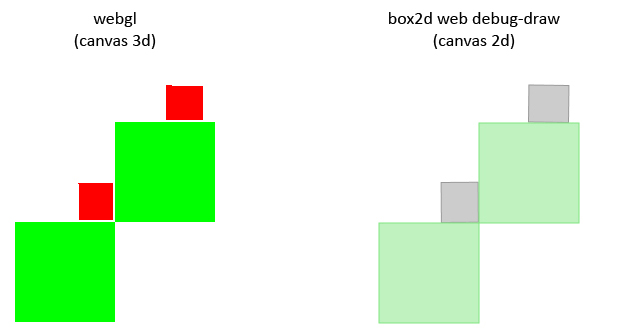
\includegraphics[scale=0.6]{images/gap_bug.jpg}
	\caption{Lücken-Bug: links WebGL, rechts box2dweb debug-view}
\end{figure}

Eine Möglichkeit zur Lösung dieses Problems, wäre es die Grafikobjekte leicht größer zu zeichnen als sie sind. Box2D bietet zudem eine Eigenschaft, mit der festgestellt werden kann, wie groß die Schutzschicht um ein dynamisches Physik-Objekt herum ist. Basierend darauf könnte man die zu zeichnende Größe des Grafik-Objekts bestimmen. Diese Aufgabe wurde jedoch noch nicht erledigt.

\subsection{Anti-Aliasing}

Bei Überprüfung dieses Lücken-Zustandes in der box2dweb-Debug-Ansicht (siehe Screenshot), sieht es so aus, als ob die Lücken dort kleiner wären. Dies hat damit zu tun, dass dort ein 2D-\textprog{canvas}-Kontext genutzt wird, bei dem - im Gegensatz zu WebGL - anti-aliasing aktiviert ist.


\chapter{Module}

Der Programmcode der Game-Engine sowie des Spiels ist innerhalb von Modulen geordnet. Diesem Pattern folgend existieren zusammengehörige Programmteile innerhalb eines eigenen Scopes und stellen nur ein vom Programmierer definiertes Interface bereit. Diese Kapselung erleichtert die Wartung des Codes und bietet weitere Vorteile. Durch das Leben innerhalb eines eigenen Scopes, wird der globale Namensraum nicht unnötig verschmutzt. Daraus folgt zudem, dass ein Modul die eigenen Abhängigkeiten klar definieren muss, anstatt innerhalb des Codes auf eine beliebige globale Variable zuzugreifen.\\
Ein weiterer Vorteil besteht darin, dass Module, sofern sie dasselbe Interface bereitstellen, austauschbar sind. 

Ich habe das Modulsystem mit Blick auf die Anforderungen einer Game-Engine erstellt - es jedoch auch so entwickelt, dass es der CommonJS-Modulspezifikation\footnote{\url{http://wiki.commonjs.org/wiki/Modules}} folgt. Bei \textbf{\href{http://www.commonjs.org/}{CommonJS}}\footnote{\url{http://www.commonjs.org/}} handelt es sich um ein Projekt mit dem Ziel Javascript auch in Bereichen außerhalb des Webs (z. B. Server und Desktop-Applikationen) zu einer ebenbürtigen Programmiersprache mit vergleichbarem Ökosystem zu machen.

Das Modulsystem stellt zwei wichtige Funktionen bereit: \textprog{registerModule} zum Registrieren eines Moduls sowie \textprog{require} zum Zugriff auf ein Modul.

\section{registerModule}

\begin{lstlisting}[language=JavaScript]
registerModule([string] id, [function] factory) 
\end{lstlisting}

\textprog{registerModule} nimmt zwei Argumente. Zum einen die ID unter welcher das Modul registriert werden soll. Der zweite Parameter ist eine Factory-Funktion, welche, wenn aufgerufen, das Modul erzeugt. Diese Funktion wird erst bei der ersten Verwendung des Moduls durch \textprog{require} ausgeführt.

\subsection{Die Factory-Funktion}

\begin{lstlisting}[language=JavaScript]
factory([function] require, [object] exports, [object] module)
\end{lstlisting}

Die Factory-Funktion dient der Initialisierung des Moduls. Sie erhält drei Argumente. \\
Das Erste ist die \textprog{require}-Funktion, mit Hilfe derer das Modul auf andere Module zugreifen kann. \\
Das Zweite ist das \textprog{exports}-Objekt. Dieses Objekt beschreibt das Interface, mit dem man auf das Modul zugreifen kann.
Der dritte Parameter ist das Modul selbst.

\subsection{Verwendung}

Hier ein einfaches Beispiel zur Verwendung von \textprog{registerModule}:

\begin{lstlisting}[language=JavaScript, caption=Verwendung von registerModule]
ModuleSystem.registerModule("math/add", function(require, exports, module){
	
		exports.add = function add(a, b)
			{
				return a + b;
			};
		
});
\end{lstlisting}

\section{require}

\begin{lstlisting}[language=JavaScript]
[object] require([string] id)
\end{lstlisting}

\textprog{require} dient dem Zugriff auf ein Modul. Als Rückgabewert besitzt es die API des Moduls in Form des \textprog{exports}-Objekts.

Beim ersten Aufruf eines Moduls mit \textprog{require}, wird zunächst die Javascript-Datei entsprechend der übergebenen ID geladen und ausgeführt. Innerhalb dieser Datei wird \textprog{registerModule} aufgerufen um das Modul zu registrieren. Anschließend wird die Factory-Funktion des Moduls aufgerufen und das Modul somit initialisiert. Die API (das \textprog{exports}-Objekt) wird zwischengespeichert um es bei den künftigen Aufrufen von \textprog{require} zurückzuliefern.

\textprog{require} kann sowohl mit relativen, als auch absoluten Pfaden arbeiten. Ein absoluter Pfad beginnt mit einem ''/'' und bezieht sich auf den Root-Pfad des Modulsystems.

Die \textprog{require}-Funktion, welche der Factory-Funktion übergeben wird, lädt, sofern kein absoluter Pfad angegeben wird, die Module relativ zum Verzeichnis des aktuellen Moduls. Ist das Modul beispielsweise ''/dir/module'', so würde ''require('other')'' versuchen auf das Modul ''/dir/other'' zuzugreifen.

\subsection{Verwendung}

Hier ein einfaches Beispiel zur Verwendung von \textprog{require}:

\begin{lstlisting}[language=JavaScript, caption=Verwendung von require]
var add = require("/math/add").add;

alert("7 + 3 = " + add(7, 3));
\end{lstlisting}

\section{Dynamisches Laden von JS-Skripten}

Ein Aufruf von \textprog{require} ist immer synchron, unabhängig davon, ob das Modul zuvor schon geladen wurde oder nicht. Dies bedeutet, dass das dynamische Laden und Ausführen der entsprechenden Javascript-Dateien beim ersten Aufruf von \textprog{require} ebenso synchron, sprich: blockierend, erfolgen muss.

Dieser Prozess geschieht durch das dynamische Erzeugen von HTML \textprog{script}-Tags. 
Dabei gibt es zwei Möglichkeiten: \\
\textbf{a)} man lädt den Text eines Skripts per \textbf{synchronem} HTTP-Request (damit blockiert wird) und setzt ihn als Inhalt eines neu erzeugten \textprog{script}-Tags.\\
\textbf{b)} man erzeugt ein neues \textprog{script}-Element und setzt dessen \textprog{src}-Attribut auf den Pfad der zu ladenden Javascript-Datei.

Variante \textbf{a} bietet den Vorteil, dass der Javascript-Code sofort bei Einfügen des Elements ins DOM blockierend ausgeführt wird. Leider geht jedoch die Information, woher der Code kommt, sprich der Dateipfad, verloren, was das Debugging des Programmcodes z. B. mit Hilfe der Firefox-Extension \textbf{\href{http://getfirebug.com/}{Firebug}}\footnote{\url{http://getfirebug.com/}} erschwert.

Bei Variante \textbf{b} bleibt die Datei-Information erhalten, sodass man mit Hilfe von Firebug durch die Dateistruktur navigieren kann. Nach mehreren Tests und Variationen musste ich jedoch feststellen, dass ein blockierendes Ausführen des Codes mit dieser Variante nicht direkt möglich ist. Selbst das Fehlen des HTML5-\textprog{async}-Attributs des \textprog{script}-Elements, wodurch das Element angewiesen werden soll das Skript synchron zu laden, scheint beim dynamischen Erzeugen von \textprog{script}-Elementen keinen Unterschied zu machen, wahrscheinlich, weil dieses Attribut lediglich für den HTML-Parser beim initialen Parsen des Dokuments gedacht ist. \\
Da ich nicht auf Debugging-Möglichkeiten in Form von Firebug verzichten wollte, entwickelte ich einen ''unschönen'' Workaround. Bei Erzeugung des \textprog{script}-Elements setze ich einen EventListener für das \textprog{load}-Event, welches die eigens hinzugefügte Eigenschaft \textprog{loaded} auf \textprog{true} setzt, sobald das Skript erfolgreich geladen und ausgeführt wurde. Sofort nach Erzeugung des Elements, welches in jenem Moment das asynchrone Laden der JS-Datei startet, beginne ich die weitere Ausführung des Codes zu blocken, so lange die \textprog{loaded}-Eigenschaft des Elements nicht \textprog{true} ist. Die einzige Möglichkeit, die Javascript mir dazu bietet, ist die wiederholte Erzeugung eines synchronen HTTP-Requests zu einer beliebigen Datei. Dieser Workaround wird nur zu Debugging-Zwecken verwendet.

\subsection{Optimierung}
Das rein dynamische Laden der Module ist für die prototypische Entwicklung zwar sehr bequem, kann jedoch zu einem unflüssigen Verlauf des Spiels führen, wenn der Code für Module erst mitten in der Ausführung durch einen Aufruf von \textprog{require} geladen und ausgeführt wird.

Das Modulsystem lässt es daher zu die Modul-Dateien mit normalen \textprog{script}-Elementen im HTML-Code der Website zu laden und somit schon an dieser Stelle die Module zu registrieren, sodass beim ersten Aufruf von \textprog{require} die bereits geladene Modul-Factory-Funktion lediglich ausgeführt werden muss. Ist dieser Prozess immer noch zu zeitaufwendig, kann man selbstverständlich bereits zu Beginn der Applikation bzw. vor Start der GameLoop \textprog{require} für alle notwendigen Module aufrufen um diese korrekt zu initialisieren.

GraphicsCore, WebGL, canvas, Shader, Texturen, GraphicPlugins
AudioCore

EventThrower

Testgame, Spielprinzip

Auswertung